% !TeX root = ../main.tex
\section{Evaluation}
\label{sec:evaluation}
\flushbottom


\subsection{Experimental Setup}
\textbf{Hardware.}
We evaluate on one NVIDIA A100 80~GB PCIe GPU with a local HDD-backed RAID volume.
Expert weights remain in FP16.
Each comparison fixes the primary HBM and CPU residency budgets; host memory also holds mirrors of HBM-resident experts and staging buffers.

\textbf{Models and workloads.}
The main comparison covers Mixtral-8$\times$7B and Qwen2-57B-A14B.
The workloads are WikiText-2, GSM8K, and HumanEval.
Unless stated otherwise, each uses eight prompts of 128 input tokens and 128 output tokens.
We serve requests sequentially with batch size one and greedy decoding.
Methods receive matched prompts and residency budgets within each comparison.

\textbf{Baselines.}
We compare MECC with on-demand Streaming, Fiddler, MoE-CORE, MoE-Infinity, SSD-LLaMA, and FlashMoE-RF~\cite{fiddler,core,moeinfinity,ssdllama,flashmoe}.
Streaming loads each requested expert from the backing store when it is needed.

\textbf{Metrics.}
TTFT measures time to the first token; TPOT averages the time per subsequent token.
Both include computation and expert delivery, and we average latency across prompts.
For each model, workload, and metric, Figures~\ref{fig:performance} and~\ref{fig:performance_qwen} report $T_{\mathrm{Fiddler}}/T_{\mathrm{method}}$; values above one indicate lower latency than Fiddler.

\begin{figure}[H]
\centering
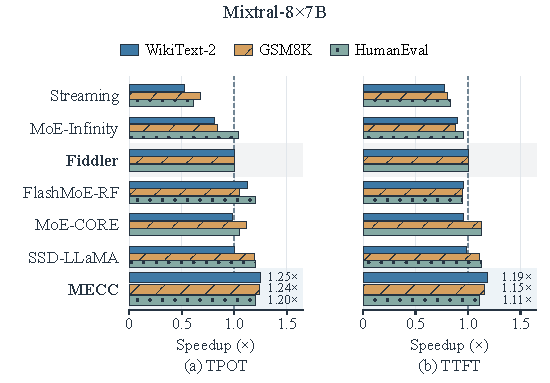
\includegraphics[width=\columnwidth]{figures/fig07_main_mixtral_compact.pdf}
\par\nointerlineskip
\caption{TPOT and TTFT comparison on Mixtral-8$\times$7B.
Speedup is relative to Fiddler under the matched model, workload, and metric; higher is better. Methods follow a common order within both panels.}
\label{fig:performance}
\vspace{5pt}
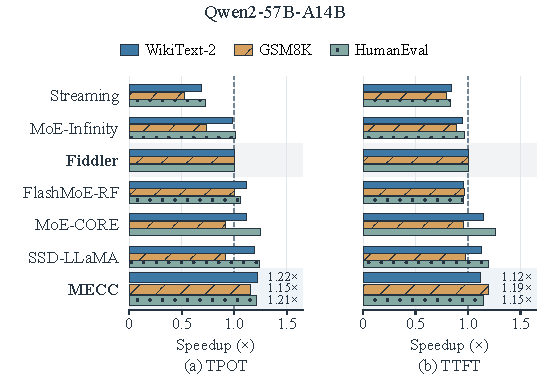
\includegraphics[width=\columnwidth]{figures/fig08_main_qwen_compact.pdf}
\par\nointerlineskip
\caption{TPOT and TTFT comparison on Qwen2-57B-A14B.
Colors and method order match Figure~\ref{fig:performance}; speedup is relative to Fiddler.}
\label{fig:performance_qwen}
\end{figure}

\subsection{End-to-End Performance}
\textbf{Main comparison.}
Across the three workloads, MECC achieves 1.20--1.25$\times$ TPOT and 1.11--1.19$\times$ TTFT speedup over Fiddler on Mixtral-8$\times$7B (Figure~\ref{fig:performance}).
On Qwen2-57B-A14B, the corresponding ranges are 1.15--1.22$\times$ and 1.12--1.19$\times$ (Figure~\ref{fig:performance_qwen}).
The bars report separate comparisons for each workload and response stage; a TPOT ratio and a TTFT ratio do not share a latency denominator.
MECC exceeds the Fiddler reference in every displayed model--workload pair for both metrics.
The gain changes with the input and response stage, indicating that a single aggregate ratio would conceal useful differences in expert demand.

\textbf{Generation and first-token latency.}
During decoding, repeated expert requests may hit in HBM, use a host-resident copy, or require another HDD read.
MECC retains a displaced GPU expert in the host slot released by promotion, making that copy available to later requests.
If that expert is selected again after leaving HBM, its host copy can serve the request without another HDD read.
The access also updates the recency order, so future replacement responds to the observed sequence rather than only the initial analysis ranks.
For TTFT, the initial resident set and reuse among input tokens also affect the time to the first response.
Prefill may select several experts before any output token is produced; a cold expert on this path can delay the first response even when later decode requests benefit from reuse.
The two panels therefore expose different effects of placement and retention; the component controls below examine them separately.

\textbf{Model and workload response.}
On Mixtral, MECC's TPOT ratios are close across the three inputs, while its TTFT gain declines from WikiText-2 to HumanEval.
Qwen2 shows a different phase response: GSM8K has the smallest TPOT gain but the largest TTFT gain for MECC among its three workloads.
The two models have different expert organizations, so a fixed byte budget covers different numbers of experts and different portions of routed demand.
Within a model, the order and spacing of requests determine whether a previously used expert remains in HBM, survives in CPU memory, or must be fetched again from HDD.
These factors provide a mechanism for the workload-dependent trends without requiring the same relative gain in prefill and decode.
Because TPOT and TTFT use separate Fiddler denominators, their ratios describe improvement within each stage rather than a comparison of absolute stage durations.

\textbf{Mechanism context.}
The baselines differ in where they execute experts and how they choose residents: Fiddler may compute on the CPU, MoE-CORE allocates capacity by layer, MoE-Infinity tracks request history, SSD-LLaMA manages three storage tiers, and FlashMoE uses learned replacement~\cite{fiddler,core,moeinfinity,ssdllama,flashmoe}.
MECC's initial plan allocates slots to layers according to analyzed expert demand, while serving accesses revise membership inside those allocations.
The promotion rule connects the two resident tiers: the expert leaving HBM retains a host path through its existing mirror instead of becoming an immediate cold miss.
The main figures include the combined cost of lookup, movement, execution, and replacement; they do not isolate these steps.
Figures~\ref{fig:ablation_components} and~\ref{fig:ablation_traffic} separate the placement, retention, and delivery contributions using the same component sequence.

\textbf{Delivery path.}
An HBM hit needs no weight transfer; a CPU hit copies weights to the GPU; an HDD miss adds a host read before that copy.
During prefill, a cold read may overlap execution of a resident expert, but its consumer waits for read and copy completion.
Thus, request-source counts alone do not determine the exposed latency, a distinction examined in Figure~\ref{fig:ablation_traffic}.

\clearpage
\subsection{Ablation Study}
We add placement, joint retention, and delivery scheduling in sequence, then measure request sources and exposed time under the same configurations.
\begin{figure}[H]
\centering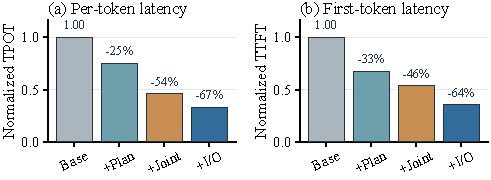
\includegraphics[width=\columnwidth]{figures/fig09_ablation_startup.pdf}
\par\nointerlineskip
\caption{Component addition and initialization amortization. (a) Adding placement, joint retention, and delivery scheduling. (b) Initialization plus generation over output length.}
\label{fig:ablation_components}
\end{figure}
\textbf{Component addition.}
Figure~\ref{fig:ablation_components}(a) shows the TPOT change after each component is added.
The largest reduction follows joint retention, which keeps a displaced GPU expert in the host tier.
The plan changes the starting residents; joint retention then changes which experts remain accessible after a GPU replacement.
This distinction matters because a useful initial set alone cannot preserve an expert once subsequent requests displace it.
Panel (b) includes initialization cost: over $n$ output tokens, its amortized contribution is $T_{\mathrm{init}}/n$ per token.

\begin{figure}[H]
\centering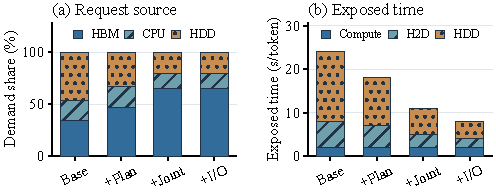
\includegraphics[width=\columnwidth]{figures/fig10_traffic_exposure.pdf}
\par\nointerlineskip
\caption{Expert request sources and exposed time across the same component sequence.}
\label{fig:ablation_traffic}
\end{figure}
\textbf{Traffic and delivery.}
Figure~\ref{fig:ablation_traffic}(a) shows the fraction of expert requests served from HBM, CPU, and HDD after each component is added.
Panel (b) breaks exposed time into computation, host-to-device transfer, and HDD access.
The final delivery step changes exposed time without changing the request-source fractions, separating scheduling effects from changes in cache residency.
Thus, a lower HDD demand share and a shorter exposed HDD interval are distinct effects: the former changes where requests hit, while the latter changes how much of a required read remains on the critical path.

\subsection{Sensitivity Analysis}
\begin{figure}[H]
\centering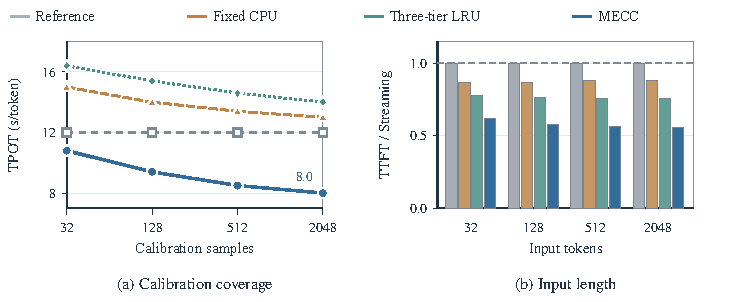
\includegraphics[width=\columnwidth]{figures/fig11_calibration_input.pdf}
\par\nointerlineskip
\caption{Sensitivity to analysis samples and input length. TTFT uses the Streaming reference at each input length.}
\label{fig:workload_sensitivity}
\end{figure}
\textbf{Analysis and request shape.}
Figure~\ref{fig:workload_sensitivity}(a) increases the number of analysis samples from 32 to 2048; TPOT decreases from 10.8 to 8.0~s/token.
Panel (b) reports TTFT relative to Streaming at each input length, so each point uses a length-matched denominator.
The TPOT curve flattens as the analysis set grows, consistent with later samples making smaller changes to the selected initial residents.

\begin{figure}[H]
\centering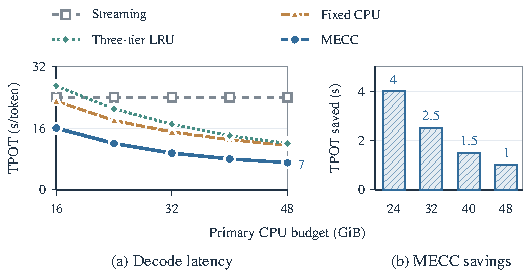
\includegraphics[width=\columnwidth]{figures/fig14_quota_targets.pdf}
\par\nointerlineskip
\caption{CPU capacity sensitivity. (a) TPOT at a fixed HBM budget. (b) Savings from each additional allocation.}
\label{fig:capacity_sensitivity}
\end{figure}
\textbf{Host capacity.}
Figure~\ref{fig:capacity_sensitivity} increases primary CPU residency from 16 to 48~GiB at a fixed HBM budget; MECC TPOT falls from 16 to 7~s/token.
The first 8~GiB increment saves 4~s/token, whereas the last saves 1~s/token.
The diminishing reduction is consistent with additional slots covering less frequently reused experts.

\begin{figure}[H]
\centering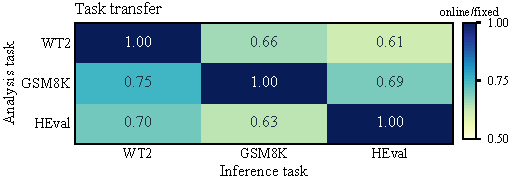
\includegraphics[width=\columnwidth]{figures/fig15_profile_mismatch.pdf}
\par\nointerlineskip
\caption{Task transfer. Rows select the analysis task; columns select the inference task. Both panels share a TPOT scale.}
\label{fig:task_transfer}
\end{figure}
\textbf{Task transfer.}
In Figure~\ref{fig:task_transfer}, rows specify the analysis task and columns the inference task.
Across the six off-diagonal pairs, online membership reduces mean TPOT from 14.00 to 9.38~s/token, a 33.0\% decrease; the diagonal entries are unchanged.
For the HumanEval inference column, the largest fixed-residency value falls from 16 to 9.8~s/token with online updates.
An access to an expert outside the initial set admits it to the resident hierarchy; later requests can then reuse the new placement.
The unchanged diagonal cells and reduced off-diagonal values separate adaptation to a changed task from simply increasing the slot budget.

\flushbottom
